This section focuses on the mirrors forming the arm cavities of the interferometer (IM and EM). Those optics, also called test masses, are the largest \tcb{(comment sthild:) by dimension} and most critical ones whose displacement noise can directly degrade the  \tcb{(comment sthild:) measurement of the } gravitational waves signals.

To ensure the best optics, the three ingredients of a mirror: substrate, polishing and coating will have to use state of the art technologies. An overview of current achievements and the core optics strategy for ET is presented in the following sections. The working temperature of the optics \tcb{(comment sthild:) better say "The temperature at which the mirror is operated  has ..." } have a strong impact on the technological choices to be made. 

\subsubsection{The substrate materials}

The substrate of the large \tcb{(comment sthild:) replace 'large' by 'ET main' } optics must meet some drastic \tcb{(comment mlorenzini: replace specifications with requirements)} specifications in term\tcb{s} of optical and mechanical specifications, moreover it should be available in large sizes with surfaces polished to the atomic level. Due to such constraints, \tcb{(comment sthild:) only a }few specific materials can be considered: fused silica for room temperature interferometer and silicon for cryogenic temperatures.\\

\paragraph{Fused silica} is the substrate of choice for all the current room temperature interferometers.  Due to its \tcb{(comment mlorenzini: Remove 'extensive') } extensive
use for first and second generation gravitational wave detectors, this material has been extensively characterised at room temperature. Moreover the polishing and coating are now well mastered for this material \cite{pinard2017mirrors}.

The operating wavelength of room temperature ET will be 1064~nm, the same as current advanced interferometers and well within the transparency region of fused silica. At this wavelength fused silica exhibits very low bulk optical absorption (below 1 ppm/cm) with high homogeneity of refractive index (relative optical path length < 0.1~nm/cm over the central part) and very low birefringence (around 1~nm/cm \cite{Degallaix:Large_optics_19}). The material can be isotropic in 3 dimensions which is ideal for the central beansplitter where laser beams are crossing the substrate at different angles.

In addition to its outstanding optical properties, fused silica presents a very low Brownian thermal noise at room temperature. Additionally, there exist techniques to fabricate quasi-monolithic suspensions based on pulled fused silica fibres and silicate bonding to further reduce the suspension thermal noise. These techniques have demonstrated their reliability and performances for years in the GEO600 detector \cite{plissi1998aspects} and so have been successfully implemented in the LIGO and Virgo detectors \cite{robertson2002quadruple,lorenzini2010monolithic}.

As a risk reduction for ET, the upgrade of Advanced Virgo, called Advanced Virgo+, will use test masses in fused silica of diameter 55~cm weighting 100~kg, that would be an essential step towards the optics for ET-HF which will be in the same material and with a diameter of 62~cm for 200~kg. 

In a nutshell, fused silica for large optical substrates presents the best optical and mechanical performances at room temperature and with very limited risks.\\


\paragraph{Silicon} is the favorite candidate material for the test masses for the cryogenic interferometer ET-LF. Compared to fused silica (and sapphire), silicon is not transparent at 1064~nm and so the operating wavelength of the detector has to be shifted to 1550~nm. 

Silicon has excellent mechanical and thermal properties and is easily available in relatively high quality due to the large market of the semiconductor industry. The coefficient of thermal expansion is zero at two special temperatures around 18~K and 125~K \cite{lyon1977siliconexpansion}. At these temperatures the contribution of thermo-elastic noise will therefore vanish. The mechanical loss of silicon has been studied by Q-factor measurements. It was experimentally shown that silicon bulk samples can reach mechanical losses as low as $1 \times 10^{-9}$ at 10~K. \cite{mcguigan1978siliconQ}.

The maximum available diameter and purity of silicon depends on the fabrication process. The two main growing processes for single crystal silicon used by the semiconductor industry are the Czochralski (CZ) and the Float Zone (FZ) methods. CZ silicon is grown from a silicon melt in a silica crucible. It results in relative large samples with a reasonable purity. The most dominant impurities in undoped CZ-grown silicon are carbon (typically 10$^{-18}$ cm$^{-3}$) and oxygen (typically up to 10$^{-19}$ cm$^{-3}$). 

In contrast, FZ silicon contains the same impurities but in much smaller concentrations (up to 10$^{-3}$ times smaller\tcb{(comment MGranata:) I would rather say "10$^{3}$ times smaller"}). During the FZ growth process, single or poly-crystalline silicon is remelted by means of inductive heating in vacuum or under an inert atmosphere. Impurities dissolve better in the melt than in the solid part. The re-crystallised material has therefore a higher purity than the initial one. By slowly sweeping the melt from one end to the other it is possible to purify in steps. The mechanism of inductive heating sets limits to the current production setups and leads to smaller available samples.

Using the CZ growth technique, silicon ingots up to 45~cm of diameter can be produced however 30~cm is still the dominant \tcb{(comment mlorenzini: perhaps replace "dominant" with "most common") } wafer diameter in the semiconductor industry. For FZ silicon the diameter is currently limited to 20~cm.

In the recent years, motivated by the possible use of silicon as test mass material, the optical properties of silicon have been thoughtfully characterised. Regarding the bulk optical absorption at 1550~nm, it was demonstrated the direct link between impurities concentration and the absorption \cite{degallaix2013abs_silicon}. For FZ silicon, absorption below 5~ppm/cm has been measured which is compatible with the ET-LF requirement. During the absorption studies, excess optical absorption at the surface of silicon was reported \cite{khalaidovski2013indication} which is likely linked to the polishing techniques used and not intrinsic to the material \cite{bell2017Sisurf}. According to the latest measurement \tcb{(comment mlorenzini: Perhaps a reference, if possible, should be added )}, magnetic Czochralski (mCz) growth technique would be the most suitable approach for ET as it can combine large diameter ingot (45~cm) with very low impurities since absorption around 20~ppm/cm has been achieved on one sample.

Thanks to the very low intensity of the laser beam in ET-LF, non linear effects such as two photon absorption \cite{bristow2007two} or Kerr effect are expected to be negligible in silicon.

Other caracterisations done in the framework of the Einstein Telescope include the measurement of thermo-optic coefficient at low temperature \cite{komma2012SithermoOptic} which is essential to derive the thermal lensing magnitude and the substrate thermo-refractive noise and also the birefringence \cite{kruger2015birefringenceSi} which is in the same order of magnitude as for sapphire. 

The choice of silicon substrate for ET-LF will be validated when it could be demonstrated that this material can come in large size (diameter of 450~mm\tcb{(comment MGranata:) everywhere else in this section, diameters are given in cm ----> 45 cm}) together with a very low optical absorption (order of several\tcb{(comment MGranata:) I would say "few" rather than "several"} ppm/cm) at 1550~nm. Silicon ingot made with mCz seems to meet those specifications on some samples but the repeatability has yet to be proven.

A backup substrate choice could be sapphire \tcb{(comment MGranata:) I would remove "as a candidate material for ET-LF", redundant here}as a candidate material for ET-LF. Sapphire is already used in the Japanese cryogenic interferometer KAGRA and hence extensive experience has been acquired on operating those mirrors \cite{Akutsu_2019} in cold conditions. As for silicon, very large sapphire boules \tcb{(comment mlorenzini: Consider replacing "boules" with "masses" or "bulks")} with excellent optical properties still have to be demonstrated.

\subsubsection{Surface polishing achievement}

The polishing capability will depend on the substrate material. Polishing of fused silica is well mastered thanks to current generation of room temperature interferometers and hence presents little risks. For the Einstein Telescope, the same flatness and roughness that was achieved \footnote{flatness inferior to 0.5~nm RMS and roughness below 0.1~nm RMS on the central part \cite{pinard2017mirrors}.} for Advanced detectors will be enough, albeit on a larger area. Due to the heavier substrate, special handling tools will have to be manufactured but according to the polishing companies, there is no showstopper. The large end mirrors of Advanced Virgo+ with a diameter of 550~mm and weighting 100~kg is \tcb{(comment mlorenzini: Replace "is" with "represent") } a pertinent pathfinder before the procurement of the ET mirrors.

Polishing of silicon does not carry any difficulties as this substrate material is heavily used for X-ray mirrors. Experiences from polishing companies indicate that silicon could be polished the same way as fused silica and similar performances on the flatness could be achieved (using also ion beam figuring to reach sub-nanometer flatness). The very low roughness is more challenging but 0.2 nm RMS could be achieved and is acceptable for ET. In a nutshell   \tcb{(comment nchriste:) In short }, the polishing of the large silicon substrates of ET is within the reach of the current technology.

Sapphire - the backup choice for low temperature test mass - is one of the hardest known material and has always been very difficult to polish. However, as demonstrated by the KAGRA detector, the outstanding surface quality of fused silica could also be reproduced on sapphire \cite{hirose2014sapphire} but at larger time and money-wise costs.

In summary, the polishing of the large substrates of the Einstein Telescope is within the current polishing capability and as such does not pose any challenge.

\subsubsection{Coating procurement}

Thin optical coatings, a few microns in thickness, must be added to the surfaces of the inteferometer mirrors to make them highly reflective. Since the thermal noise from these coatings will already limit the sensitivity of current room-temperature detectors at their most sensitive frequencies\tcb{(comment MGranata:) maybe recalling some references here would be useful, like the reference papers on Advanced Virgo and Advanced LIGO (Acernese et al CQG 2015, Abbott et al CQG 2015)}, it is essential to reduce coating thermal noise to achieve ET design sensitivity.

Highly-reflective coatings are usually composed of a stack of layers of alternating refractive index, with each layer having an optical thickness of a quarter of a wavelength. Using more layers or materials with a larger difference in refractive index \tcb{(comment MGranata:) I would rather say "with a larger refractive index contrast" (which is a ratio, not a difference)}results in higher reflectivity. Different layer thicknesses may be used to reduce thermo-optic noise\tcb{(comment MGranata:) a reference here?}, to optimise the coating thermal noise \tcb{(comment MGranata:) maybe add a reference here, A. E. Villar {\it et al.}, {\it Phys. Rev. D} {\bf 81}, 122001 (2010).}or to provide reflectivity at more than one wavelength.

The amplitude spectral density (ASD) of coating thermal noise can be approximated by\tcb{(comment MGranata:) maybe add a reference here, G. M. Harry {\it et al.}, {\it Class. Quantum Grav.} {\bf 19}, 897 (2002).}

\begin{equation}
x(f)=\sqrt{\frac{2 k_B T}{\pi^2 f}\frac{d}{w^2}\phi\left(\frac{Y_{\rm coat}}{Y^2_{\rm sub}} +\frac{1}{Y_{\rm coat}} \right)}\,
\label{equ:CTN}
\end{equation}

\noindent where $k_{\rm B}$ is the Boltzmann constant, $T$ the mirror temperature, $f$ the frequency, $d$ the coating thickness, $w$ the radius of the laser beam on the coating and $\phi$ the mechanical loss of the coating. $Y_{\rm sub}$ and $Y_{\rm coat}$ are the Young's moduli of the substrate and coating materials. This formula assumes that the bulk and shear mechanical loss angles of the coating are identical, that the mechanical loss is frequency independent and that the Poisson ratios of the coating and the substrate are zero. Further discussion of the validity of some of these assumptions is given below. While Eqn~\ref{equ:CTN} is often used to estimate thermal noise, it should be noted that the result can be as much as 30$\%$ different from the result given by the full formula which accounts for field penetration into the coating and does not neglect the Poisson ratios.

The main approaches to reducing coating thermal noise can be identified from Eqn~\ref{equ:CTN}:
\begin{itemize}
	\item Reducing the loss of the coating materials (lower $\phi$) e.g. by varying deposition parameters, post-deposition treatments or by developing alternative coating materials
	\item Reducing the required thickness of the coating (lower $d$) - using materials with a large contrast in refractive index results in fewer pairs of layers being required to provide the same reflectivity.
	\item Reducing the mirror temperature (lower $T$). While this directly reduces the thermal energy in the system, care is needed as the mechanical loss of many materials is strongly temperature dependent.
    \item Increasing the interferometer laser beam radius on the mirrors (larger $w$). This averages thermal motion of the coating over a larger area, reducing the noise. However, the laser spot size is limited by the radius of the mirror to keep scattering / diffraction losses at the edge of the mirror to an acceptable level.
\end{itemize}
\tcb{(comment MGranata:) I would suggest to add here the following sentence, right after the bullet list:
"Furthermore, the lowest coating thermal noise occurs when the coating Young’s modulus is matched to that of the substrate [x]."
[x] G. M. Harry {\it et al.}, {\it Class. Quantum Grav.} {\bf 19}, 897 (2002).}
Current detectors use coatings formed from alternating layers of silica (SiO$_2$) and titanta-doped tantala (TiO$_2$-Ta$_2$O$_5$)~\cite{Pinard2017,Flaminio2010,Harry2007}\tcb{(comment MGranata:) please add here the following reference:
M. Granata et al., https://doi.org/10.1088/1361-6382/ab77e9 . NB: Ref [131] is surely interesting for many reasons but is not about the actual coatings of aLIGO and AdV}. The loss of these coatings has been observed to increase at cryogenic temperatures, to a peak at $\sim$30\,K~\cite{Granata2013}. Similar loss peaks have been observed in single layers of SiO$_2$~\cite{Martin2014} and TiO$_2$-Ta$_2$O$_5$~\cite{Martin2009}, with the magnitude of the loss and the temperature at which loss peaks occur being strongly dependent on post-deposition annealing temperature~\cite{RobieThesis,Martin2010}. Current coatings are therefore not suitable for use at low temperatures \footnote{One study of an ion-beam sputtered silica/tantala coating did not show evidence of a loss peak at low temperature: however, the level of loss is still higher than required for ET-LF~\cite{Hirose2014}}.

\subsubsection{Coating thermal noise - full treatment}

Equation~\ref{equ:CTN} is an useful and convenient approximation of the magnitude of coating thermal noise. However, a material can have two independent loss angles, associated with shear deformations and `bulk' (volume change) deformations. These loss angles are assumed to be identical in Eqn~\ref{equ:CTN}: for many materials, this is unlikely to be a valid assumption. A more complete expression for coating thermal noise in terms of bulk and shear loss is given by Hong~\cite{Hong2013}. This treatment also shows that the thermal noise measured by an interferometer is more sensitive to the bulk loss angle than to the shear loss angle. For detailed thermal noise calculations, it is therefore important to know both the bulk and shear loss of the coating materials.

Equation~\ref{equ:CTN} ignores also the effect of the penetration of the laser beam into the coating stack. In reality, the sensitivity of the interferometer to thermal motion in a particular layer is dependent on that layer's position in the coating stack~\cite{Hong2013,gurkowski2010,gorodetsky2008,kondratiev2011}. While this usually results in a small correction of 10$\%$ or less, this effect must be taken into account when making accurate thermal noise predictions.

\subsubsection{Coating requirements}

\paragraph{ET-LF}
To meet the goal of a factor of 25 improvement in sensitivity over aLIGO design sensitivity at 10\,Hz, ET-LF requires a reduction in coating displacement thermal noise by at least a factor of 10 with respect to the aLIGO design  sensitivity. Some of this improvement can be obtained from operating at low temperature and through the use of larger laser beam spots on the mirrors. The remainder of the improvement will need to come form the coating materials themselves. The most relevant material properties are the coating mechanical loss and the coating thickness (which is determined by the combination of refractive indices of the materials used in the coating stack). However, the elastic modulus of the coating (and of the mirror substrate) also contributes to the magnitude of the coating thermal noise.

For operation at 10\,K, after  accounting for the effect of  temperature and the effect of \tcb{(comment mlorenzini: Consider removing "the effect of")} larger beam size in ET-LF, a reduction in coating thermal noise ASD \tcb{(comment MGranata:) has this acronym been already used/explained above?"}by a factor of 1.24 must be obtained from improvements to the \tcb{(comment mlorenzini: Consider replacing "improvements to the" with "improved")}coating materials. When taking account of the substrate modulus effects, and assuming all coating properties except mechanical loss remain the same as in aLIGO, this translates to a factor of 3.8 reduction in coating loss compared to the loss of SiO$_2$/TiO$_2$:Ta$_2$O$_5$ at 10\,K.

\paragraph{ET-HF}
The target for ET-HF is a factor of 3.2 reduction in coating thermal noise ASD at 100\,Hz compared to aLIGO design sensitivity. Accounting for the slightly larger laser beam in ET-HF, this sets a requirement of a reduction in ASD by a factor of 2.7 from the coating materials. If we assume all coating properties except the mechanical loss remain identical, then a reduction in mechanical loss by a factor of 7.1 with respect to the aLIGO coatings would be required.

\paragraph{Other requirements}
In addition to meeting these thermal noise requirements, the coatings must have low optical absorption and low scattering. Low absorption is essential to minimise the heat-load on the cryogenic mirror. A target of 5\,ppm absorption was set in the original design study. Significantly lower absorption -- perhaps similar to the sub-ppm absorption of the current aLIGO and Advanced Virgo coatings -- may be required to enable the design of suspension fibres which can successfully extract the laser power absorbed by the mirror while also having acceptably low thermal noise~\cite{Cumming_2013}. Further studies in this area are likely to be required as detailed suspension designs are developed. 
For ET-HF, the coating optical absorption is also critical to limit the thermal expansion of the surface of the mirrors. The same absorption limit of 0.5~ppm similar to current detector will still hold.

Low scattering is required to minimise the optical round trip loss from the arm cavities and to prevent scattered light picking up additional phase noise (e.g. by reflection from the non-isolated beam tube) and coupling back into the interferometer beam. The target for scattering as optical loss is in the order of 10-20~ppm of loss per mirror.


\subsubsection{Coating design solutions}

\paragraph{multimaterial coatings} -- The use of so-called multimaterial coating designs has been proposed to enable the use of coating materials with higher optical absorption than can be tolerated in a traditional 2-material design~\cite{Yam2015,multimaterial2015}. In a multimaterial coating, the top few coating layers are made from low-absorption materials e.g. silica/tantala. These layers reflect the majority of the incident laser power, reducing the light intensity in the coating to a level where higher-absorption materials (e.g. aSi, in combination with a low-index material) can be tolerated in the lower part of the stack. This allows the low mechanical loss of materials such as aSi to be exploited, without significantly increasing the total absorption of the coating stack.

\begin{figure}
	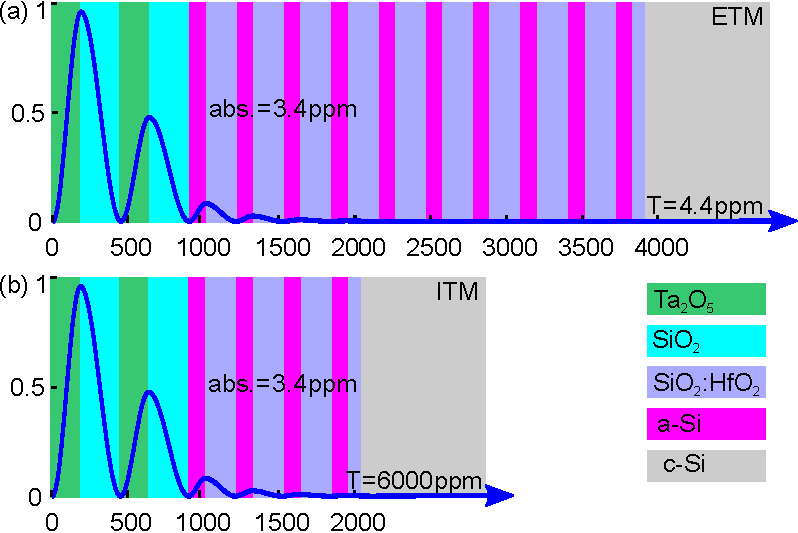
\includegraphics[width=12cm]{Detector/Optics/CoreOptics/Images/EFI_ETM_ITM_2.pdf}
	\caption{A multimaterial coatings design for (a) an ETM and (b) and ITM. This design uses an upper stack of SiO$_2$/Ta$_2$O$_5$ on top of a SiO$_2$:HfO$_2$/aSi lower stack~\cite{Craig_2019}. The blue lines show the electric field intensity as a function of depth in the coating.}
\label{fig:coatings:mulitmat}
\end{figure}

Several possible multi-material designs have been proposed to date~\cite{Steinlecher_2017,ion_plating,Pan_2018,Birney_2018,Craig_2019}\tcb{(comment MGranata:) there are 2 undefined references here}, including one that theoretically just meets the ET-LF coating thermal noise target for an optical absorption of 3.4\,ppm~\cite{Craig_2019}. This coating design relies on a level of absorption in aSi films which has been observed~\cite{Birney_2018}\tcb{(comment MGranata:) undefined reference here}, but has not yet been demonstrated reproducibly or on the scale required for ET.

Experimental verification of the performance of prototype multimaterial coatings has been reported~\cite{Gras_GWADW,Kinley_Hanlon_Warsaw} -- although it should be noted that a coating meeting the thermal noise and optical requirements of ET-LF has not been tested to date.

\paragraph{nanolayer coatings} -- Annealing at high temperatures is desirable to reduce the mechanical loss and optical absorption of many coatings: however, the onset of crystallisation (which results in higher mechanical loss and increased optical scattering) can limit the maximum tolerable annealing temperature. The nanolayer approach involves composing a single coating layer out of a stack of thinner layers of two materials~\cite{Pan2014,Sankur1989}. This substructure can inhibit crystallisation in the material, allowing higher annealing temperatures and lower mechanical loss to be achieved. This has been demonstrated for a high-index coating layer formed from a substructure of titania/silica nanolayers~\cite{Pan2014}.

More recently, it has been shown that the cryogenic loss peaks observed in silica coatings can be eliminated by using silica nanolayers separated with titania 'blocking' layers~\cite{Kuo2019}. Nanolayer coatings may therefore provide an excellent way to gain better performance from amorphous oxide materials at low temperatures. An important consideration for nanolayer coatings is to define the precision and uniformity with which each nanolayer needs to be deposited.\tcb{(comment MGranata:) I suggest adding here the following sentence: "To date, the deposition
of a full high-reflectivity coating embedding composite nanolayers has yet to be
achieved."}

\paragraph{Coating structure and mechanical loss} -- Significant progress has been made in predicting the cryogenic mechanical loss of coating materials computationally using molecular dynamics simulations~\cite{Hamadan2014,Trinastic2016,Billman2017}\tcb{(comment MGranata:) Please, add here also the following reference: F. Puosi et al., Phys. Rev. Res. 1, 033121 (2019).} and to obtain agreement with trends and magnitudes of experimental loss data.

Other structural work has shown the room-temperature loss may be correlated with medium-range order in Ta$_2$O$_5$ coatings, with more ordered structures and lower loss resulting from heat-treatment~\cite{Hart2016}. The evidence points towards the possibility that the same structural features responsible for low loss at room-temperature may be responsible for higher loss at cryogenic temperature. Raman spectroscopy studies have identified correlations between the ring structures and loss in silica coatings~\cite{granata2018correlated}. \tcb{(comment MGranata:) Please, add here also the following sentence and reference: "Very recent work has shown that a correlation exists between optical properties and internal friction in high-index oxide coatings [x]." 
[x] Amato et al., Sci Rep 10, 1670 (2020).}

Recently, evidence that specific structural units may correlate with lower loss has been found, in particular glassy structures with a high degree of corner-sharing, rather than edge or face sharing, between neighbouring tetrahedrons~\cite{Parsai2019}. This allows the structures of potential coating materials - many of which are well characterised - to be examined, and promising materials exhibiting a high degree of corner sharing to be identified and further investigated.

This increased understanding of the links between atomic structure and coating loss is a highly useful tool for developing lower-loss coatings.

\subsubsection{Possible coating materials}

\paragraph{Amorphous silicon} --  Amorphous silicon has low mechanical loss at cryogenic temperatures~\cite{Liu_1997,Murray2015}\tcb{(comment MGranata:) undefined reference here}, and has a relatively high refractive index, allowing thinner coatings -- with correspondingly lower thermal noise -- to be made. Mechanical loss as low as 2$\times10^{-5}$ has been observed in aSi coatings at room temperature and at cryogenic temperatures, and even lower loss is possible for coatings deposited at elevated temperature~\cite{Liu2014}. Elevated temperature deposition allows the aSi to form an `ideal glass' structure -- a low entropy amorphous state with very low loss.

While aSi is a very attractive material for thermal noise reasons, the optical absorption has historically been too high for use in gravitational wave detectors. Commercially grown ion-beam sputtered aSi coatings can have optical absorption of 1000 to 10000\,ppm at 1550\,nm (for a room-temperature HR stack made of aSi and SiO$_2$)~\cite{Steinlechner2016,Birney2018}. Significantly lower absorption can be achieved using a commercially available ion plating technique~\cite{ionplating}, and even lower again via electron cyclotron resonance (ECR) ion-beam sputtering~\cite{Birney2018}. The absorption of aSi tends to be significantly lower -- between a factor of 5 and 10 -- at $\sim$2000\,nm than at 1550\,nm~\cite{ionplating}. Operating ET-LF at a wavelength close to 2000\,nm may therefore be desirable to enable the use of aSi coatings for thermal noise reduction. While the absorption of the best aSi measured is still too high to allow a traditional aSi-based coating to be used, the incorporation of aSi layers into a mutimaterial coating design can allow significant thermal noise improvements while minimising the absorption contribution of the aSi layers.

aSi may also be a candidate material for a room-temperature coating. However, without further reductions in optical absorption, this is significantly more likely for a laser wavelength of 1550\,nm than for 1064\,nm, due to the higher optical absorption of aSi at 1064\,nm. However, it is interesting to note that some thermal noise reductions may be possible using aSi in a multi-material design at 1064 nm.

\paragraph{Silica coatings} \tcb{(comment MGranata:) I suggest changing the name of this paragraph to "Fluorides" and adding some text at the end of it, see below. Another option could be "Alternative cryogenic low-index layers"}-- For room-temperature detectors, efforts have largely focussed on improving or replacing the high-index coating layers which currently dominate the thermal noise. The current low-index material, silica, has a relatively low loss (as low as 4.5$\times10^{-5}$) at room temperature\tcb{(comment MGranata:) a most recent analysis shows that it is rather $\sim$2 $\times10^{-5}$: M Granata et al., https://doi.org/10.1088/1361-6382/ab77e9}. However, the loss of silica films increases significantly at cryogenic temperatures~\cite{Martin2014} - with both the structure and the magnitude of the loss being strongly dependent on post-deposition heat-treatment temperature~\cite{RobieThesis}. Therefore alternative low-index materials to silica will be required at for cryogenic coatings. A lower-loss low-index material is also likely to be required to achieve the required reduction in coating thermal noise at room temperature, although at the moment thermal noise remains dominated by the high index Ta$_2$O$_5$ layers. The room-temperature loss of silica can be further reduced by annealing at higher temperatures up to 900$^\circ$C\tcb{(comment MGranata:) please add here the reference supporting this statement: A. Amato et al., J.  Phys.: Conf. Series 957, 012006 (2018).}. In current coatings, crystallisation of the tantala layers prevents annealing above $\approx 600^\circ$C\tcb{(comment MGranata:) please add here the reference supporting this statement: A. Amato et al., J.  Phys.: Conf. Series 957, 012006 (2018).}.

\tcb{(comment MGranata:) I suggest adding the following text here: "In order to replace SiO$_2$ layers with lower-index materials, the optical properties and the internal friction of sputtered MgF$_2$ and AlF$_3$ coatings have been characterized at room temperature [Granata20]. Lower refractive index, higher optical abosrption and internal friction have been observed. Work is ongoing to characterize the impact of annealing on absorption and internal friction, at room and low temperature, for possible implementation in future cryogenic detectors like ET-LF."
[Granata20] M. Granata et al., Appl. Opt. 59, A229 (2020).}.

\paragraph{Silicon nitride} -- Silicon nitride films can have mechanical loss in the order of $1\times10^{-5}$ around 10\,K~\cite{Liu_2007} for a film on a substrate, and less than $1\times10^{-6}$ for substrate-free films~\cite{Southworth2009}. The refractive index of SiN is relatively low, making it of interest as a low-index material for use alongside aSi~\cite{Pan2017,ionplating}. Studies have shown that the exact composition of SiN films can strongly affect the refractive index, optical absorption and mechanical loss. Large enough refractive index variations can be obtained by changing the composition to potentially allow SiN to be used for both the high and low index coating layers. The optical absorption of SiN can be similar to the best aSi commercially available aSi films~\cite{Pan2017,Steinlechner2017}. A multimaterial design has been proposed to further reduce this absorption to below 5\,ppm for an HR stack ~\cite{Pan_2018}, although this design does not meet the ET-LF thermal noise requirements. 

Low mechanical loss has also been demonstrated in silicon nitride at room temperature and in sputtered films~\cite{Amato_2018}\tcb{(comment MGranata:) please replace this reference with a most recent one with updated data: M. Granata et al., Appl. Opt. 59, A229 (2020).}. Silicon nitride can withstand annealing at higher temperatures than tantala, \tcb{(comment MGranata:) please add here: "up to 900 $^{\circ}$C [x],"
[x] M. Granata et al., Appl. Opt. 59, A229 (2020).} allowing for the possibility of high-temperature annealing to produce a low loss Si$_3$N$_4$/SiO$_2$ coating.

\paragraph{Silica-doped hafnia} -- HfO$_2$ coatings have been shown to have lower cryogenic mechanical loss than SiO$_2$ and Ta$_2$O$_5$, but the material partially crystallises on annealing, resulting in poor optical properties~\cite{Abernathy_2011}. Doping HfO$_2$ with SiO$_2$ prevents crystallisation due to annealing, without increasing the cryogenic loss. With reasonably low optical absorption, SiO$_2$-doped HfO$_2$ shows promise for use as a low-index coating material to use with \tcb{(comment MGranata:) consider replacing "to use with" by "together with".}high-index aSi layers at cryogenic temperatures~\cite{Craig_2019}. This material is not of interest for ET-HF due to a relatively high room-temperature loss~\cite{CraigThesis}.

\paragraph{Alumina} Al$_2$O$_3$ coatings can have a lower mechanical loss than SiO$_2$ at cryogenic temperatures~\cite{RobieThesis}. While the refractive index is not as low as for SiO$_2$, this material may be of interest for use as a low-index material alongside materials like aSi which has a particularly high index. There has been interesting evidence that alumina coatings deposited at elevated temperatures can have significantly lower cryogenic loss than coatings which are heat-treated after deposition (REFERENCE - Abernathy?)\tcb{(comment MGranata:) I agree that a reference to the work of Abernathy et al. would be appropriate here, though -to my knowledge- only restricted-access LVC presentations are available to date?}.

\paragraph{Other amorphous coatings}
Improved amorphous oxides, with improvements being targeted using improved knowledge of the links between loss and structure, remain of interest for room-temperature coatings in particular. Options under investigation \tcb{(comment MGranata:) I can suggest a review article to be possibly cited here, covering all these options: M. Granata et al., Appl. Opt. 59, A229 (2020).}include studies of doping/mixing to increase crystallisation temperature and enable high-temperature annealing, the formation of ideal glass states using elevated temperature deposition and identifying materials with a high degree of corner-shared structural units. 

\paragraph{Crystalline coatings}

Multilayer single-crystalline coating materials can be grown epitaxially and can have very low mechanical loss. GaAs/AlGaAs crystalline coatings have been studied extensively, with a loss of 5.4$\times10^{-6}$ demonstrated at 20\,K for substrate-free resonator~\cite{Cole_2012}. Room temperature thermal noise measurements in small cavities are consistent with a coating loss of 4$\times10^{-5}$ at room temperature, and excellent optical absorption and scattering have been observed at wavelengths around 1550\,nm and 2000\,nm~\cite{Cole_2016}. AlGaAs coatings are grown on GaAs substrates, and would require to be transferred and bonded to a silica or silicon mirror - a process that is well-developed, at least for relatively small mirrors\tcb{(comment MGranata:) I do not agree with this sentence, since {Penn2019} has shown that there are relevant bonding issues even with 3" samples. I suggest replacing by "a process that might need further development"}. \greencomment{Harald:what about: "a process that needs further development for ET-sized optics."?} Currently the maximum available diameter of GaAs wafers is 20\,cm, which is not large enough for ET mirrors. However, there is now industrial interest in the production of larger GaAs wafers, \greencomment{Harald: according to a presentation of Penn 2019 expectations are that 40cm wafers would take 2 years and cost 5M\$ invest. Total equipment needed ca. 4-5y and ca. 30-40M\$} with progress towards wafer diameters up to 30\,cm.\tcb{(comment MGranata:) I suggest that at some point in this paragraph above, the risk of many defects (up to 50 microns), showed again by {Penn2019}, should be also mentioned.}

Recent work suggested that the bulk loss of AlGaAs may be significantly higher than the shear loss~\cite{Penn2019}. \greencomment{harald: Penn says, end 2019: "The excess bulk loss appears to be “all” thermoelastic"}Since the total coating thermal noise is more sensitive to bulk than to shear loss \greencomment{harald: for large beam sizes}, this requires more investigation. It should be noted that low thermal noise has been directly measured in AlGaAs coatings, although so far only on relatively small mirrors with small laser beams~\cite{Cole_2013}. 

\greencomment{harald: We should give a neutral description, with the potential, the known problems, ways to solutions and unknowns.}


GaP/AlGaP crystalline coatings have also been investigated~\cite{Lin}, with mechanical loss as low as 2.5$\times10^{-5}$ measured at 20\,K~\cite{Cumming_2015}. This material is of interest as it is lattice-matched to silicon and can be grown directly onto silicon substrates, potentially removing the need for substrate transfer (although growing a coating on an ET-sized mirror is unlikely to be feasible)\greencomment{harald: can someone qualify this statement? IBS coatings are also "grown" directly on the large mirrors.}. Measurements of an initial highly-reflective stack showed high optical absorption of 2.3$\%$~\cite{Lin_2015}: however, there may well be scope to reduce this absorption e.g. be reducing impurities in the coating materials and coating chambers.\tcb{(comment MGranata:) I suggest to add also the following: "Also, to
date, the number of layer in a high-reflectivity coating is limited [x], resulting in a limited reflectivity."
[x] Cumming et al., Class. Quantum Grav. 32, 035002 (2015).}   \tcb{(comment nchriste:) Isn't there also a problem with crystalline coatings for curved mirrors?' }

For both GaAs/AlGaAs and GaP/AlGaAs coatings, the difference in refractive index between the two materials is relatively small, and so many layers are required to provide high reflectivity, reducing some of the thermal noise improvements due to the low loss.

\paragraph{Coating deposition}
The ET mirrors will be significantly larger than current gravitational detector mirrors, and ensuring the required coating uniformity over larger diameters will require development of coating deposition facilities. This development is already underway at the state-of-the-art coating facility at the Laboratoire des Matériaux Avancés in Lyon, France. Problems with point absorbers and with bubbles - possibly of the sputtering ions used to deposit the coating - have been observed in the coatings for Advanced LIGO and Advanced Virgo: work to understand the origin of these defects and to eliminate them is a priority. \tcb{(comment MGranata:) I suggest to remove "and with bubbles" from the sentence above and to add the following sentence at the end of this paragraph: "Also, the occurrence of bubble-like defects limiting the annealing temperature of different coatings (high-index oxides) has been observed in multi-layer high-reflective stacks, work is currently ongoing also to understand and solve this issue".}

\paragraph{Strategy for ET}

Significant progress has been made towards development of coatings suitable for use at low temperatures in ET-LF. There are several highly-promising routes to meeting the coating thermal noise and optical absorption requirements. However, further study is required of the potential trade-off between coating absorption requirements, suspension thermal noise, ultimate mirror temperature and substrate thermoelastic noise -- and it seems likely that lower absorption than 5\,ppm may be required.

Achieving significant reductions in coating thermal noise at room temperature may be more challenging than at low temperature. Work in this area is ongoing, both for ET and for upgrades to the aLIGO and Advanced Virgo detectors, and there are several promising avenues\tcb{(comment MGranata:) consider replacing "avenues" by "options"}. One limitation is that some coatings which show promise for the low-temperature detector at 1550\,nm have significantly higher optical absorption at 1064\,nm, the wavelength envisaged for the room-temperature detector. Detailed studies of the benefits of operating the room-temperature detector at 1550\,nm may be of interest, as this may allow significant thermal noise reductions through the use of e.g. aSi-based coatings.

%A thin coating (few micrometers thick) is added to the polished substrates to create the optical function. For the arm cavities, the coating is a very high reflective reflector made of layers of alternate materials to form a Bragg grating. The constraints on the coating are extremely stringent as the coating must induce minimal displacement noise as well as very low optical loss.

%More specifically the coating Brownian thermal noise is the dominant source of noise and is expected to limit the sensitivity of Advanced detectors. So to further increase the detection range, intense worldwide research is currently lead to find better materials for the coating \cite{granata2019progress}. The Einstein Telescope will fully benefit from this research. 

%It is worth noting that compared to current interferometers, the impact of thermal noise on the ET noise budget is mitigated thanks to longer arm length and larger beam size.

%\paragraph{Room temperature interferometer}

%ET-HF share the same coating specifications as the Advanced LIGO + upgrade, to be operated around 2022 (a coating loss angle reduced by a factor 3 compared to current mirrors). So far no coating formulas or recipe have been found to match this requirement on large size, however people are optimistic that at the time of ET such coating would be present and well tested.


%\paragraph{Cryogenic interferometer}

%The cryogenic interferometer benefits from the lower temperature as the displacement induced by thermal noise scales as the square root of the temperature. A recent design using a multi-material approach (with the usual Ta$_2$O$_5$ and SiO$_2$ layers on top of a stack SiO$_2$:HfO$_2$ and amorphous silicon layers) has shown to meet the requirement for ET-LF \cite{craig2019mirror} for both the coating thermal noise and the optical absorption. 


\paragraph{Other core optics}

Central interferometer optics such as Power and Signal Recycling Mirrors (PRM and SRM) or beamsplitter will be smaller in size (diameter in the order of 10~cm) and at room temperature. Fused silica is hence the preferred material for the substrates. The coating will use the same materials as for ET-HF to benefit from state of the art deposition process. \tcb{(comment nchriste:) But ET-LF will be at 1.5 micron; will the coating material necessarily be the same?' } The procurement of those optics does not represent any challenges and will be straightforward.